\section{Problem Set 3}
\subsection{We are Close in Near-Circular Orbits}

\subsubsection{Initial Conditions for HCW}

We would like to use the Hill-Clohessy-Wiltshire (HCW) equations to give us a clear solution to the relative motion of the deputy satellites. However, the HCW equations assume that the motion of the depity with respect to the chief is very small compared to the orbit radius, as they rely on linearizing the non-linear equations of motion the The initial conditions for this are built over the original absolute and relative initial conditions for SV1, SV2, and SV3 that were previous defined in Table \ref{tab:abs_oe} and Table \ref{tab:relative_oe}.

The eccentricity of SV1 is already very low, as seen in Table \ref{tab:abs_oe_kepler} (and meets the conditions for applying HCW). Therefore, the orbital elements of the chief did not need to be modified. However, the relative orbital elements initial conditions create a large separation between SV1 and SV2/SV3. So the quasi-nonlinear relative orbital elements are modified to be as in Table \ref{tab:relative_oe_hcw} below. These are written in order as described in Equation \ref{eq:quasi_nonsign_roe}.

\begin{table}[h!]
\centering
\begin{tabular}{ll}
\toprule
\textbf{ID} & \textbf{HCW Conditions} \\
\midrule
SV2 & $\delta\boldsymbol{\alpha} = [0, 0, 0, 100, 0, 1000]~\text{m}$ \\
SV3 & $\delta\boldsymbol{\alpha} = [0, 0, 0, 200, 0, 800]~\text{m}$ \\
\bottomrule
\end{tabular}
\caption{Quasi-Nonsingular Relative Orbit Parameters for SV2 and Sv3 to apply for HCW}
\label{tab:relative_oe_hcw}
\end{table}

The main differences in these quasi-nonsingular relative orbital elements (and the justification for these changes), are:
\begin{itemize}
    \item $\delta\alpha$ is 0 for both SV2 and SV3, so that they have the same semi-major axes as SV1.
    \item The $\delta\lambda$ for both deputy satellites is reduced to 0. This helps reduce the separation between the deputies and the chief
    \item $\delta e_x$and $\delta i_x$ are set to zero for convenience, and to easily create a $\boldsymbol{e}-\boldsymbol{i}$ vector angle separation of $0^\circ$.
    \item $\delta e_y$ and $\delta i_y$ are set to convenient values close to the original relative orbital elements in Table \ref{tab:relative_oe}.
\end{itemize}

Based on these initial conditions, we see that the ratio of the maximum separation between spacecraft is small relative to the distance of the chief from the primary attractor.

TODO: Add something here to show this.

\subsubsection{Transforming the Initial Conditions} \label{sec:hcw_initial_conditions}
We can convert the initial conditions set in Table \ref{tab:relative_oe_hcw} to different representations. The initial conditions for the chief are not recalculated, as these have not been modified from previous sections.

\textbf{ECI and Absolute Orbital Elements} \\
Using the transformations highlighted in Equation \label{eq:quasi_nonsign_roe}, 
we convert the quasi-nonsingular relative orbital elements into absolute orbital elements. The results for SV2 and SV3 are given in Table \ref{tab:abs_oe_kepler_SV2_HCW} and Table \ref{tab:abs_oe_kepler_SV3_HCW}. The absolute orbital elements of the chief remain the same as in Table \ref{tab:abs_oe_kepler}.

TODO: Need to update these tables.

\begin{table}[h]
\centering
\begin{tabular}{cccccc} \hline
    $a$ & $e$ & $i$ & $\omega$ & $\Omega$ & $\nu$ \\ \hline 
     6944 km & 0.0016 & 99.4 $^\circ$ & 91.432$^\circ$ & -151.1$^\circ$ & -139.45$^\circ$ \\ \hline
\end{tabular}
\caption{Initial Keplerian Orbit Parameters of SV2, modified for applying HCW}
\label{tab:abs_oe_kepler_SV2_HCW}
\end{table}

\begin{table}[h]
\centering
\begin{tabular}{cccccc} \hline
    $a$ & $e$ & $i$ & $\omega$ & $\Omega$ & $\nu$ \\ \hline 
     6944 km & 0.0016 & 99.4 $^\circ$ & 91.432$^\circ$ & -151.1$^\circ$ & -139.45$^\circ$ \\ \hline
\end{tabular}
\caption{Initial Keplerian Orbit Parameters of SV3, modified for applying HCW}
\label{tab:abs_oe_kepler_SV3_HCW}
\end{table}

These Keplerian orbital elements are then converted to ECI co-ordinates using the expressions provided in Section \ref{sec:initial_ECI}. The initial ECI co-ordinates of the chief remain the same as in Equation \ref{eq:SV1_initial_ECI}. Equations \ref{eq:SV2_HCW1_ECI_initial} and \ref{eq:SV3_HCW1_ECI_initial} provide the ECI co-ordinates of SV2 and SV3. 


\begin{align} \label{eq:SV2_HCW1_ECI_initial}
    r_{0, ECI, SV2} &= \begin{bmatrix}
        -3091.3 \\
        -2937.0 \\
        -6503.8
    \end{bmatrix} km \\
    v_{0, ECI, SV2} &= \begin{bmatrix}
        -5.0008 \\
        -2.0031 \\
        4.0106
    \end{bmatrix} \frac{km}{s}
\end{align}


\begin{align} \label{eq:SV3_HCW1_ECI_initial}
    r_{0, ECI. SV3} &= \begin{bmatrix}
        -3091.4 \\
        -2937.0 \\
        -6503.7
    \end{bmatrix} km \\
    v_{0, ECI, SV3} &= \begin{bmatrix}
        -5.0009 \\
        -2.0029 \\
        4.0107
    \end{bmatrix} \frac{km}{s}
\end{align}


\textbf{Relative Position and Velocity in Chief's RTN frame, Orbital Element Differences} \\

Since the initial conditions of SV1, SV2, and SV3 are known, we can find the positions and velocities of SV2 and SV3 in SV1's RTN frame using the equations highlighted in Section \ref{sec:nonlinear_rel_eom}. These are provided below in Equations \ref{eq:SV2_HCW_RTN_init} and \ref{eq:SV3_HCW_RTN_init}.

\begin{align} \label{eq:SV2_HCW_RTN_init}
    r_{0, RTN. SV2} &= \begin{bmatrix}
        0.3256 \\
        -0.4989 \\
        -0.5971
    \end{bmatrix} km \\
    v_{0, RTN, SV2} &= \begin{bmatrix}
        -2.0102 \\
        -5.8056 \\
        -7.7372
    \end{bmatrix}\cdot 10^{-4} \frac{km}{s}
\end{align}

\begin{align} \label{eq:SV3_HCW_RTN_init}
    r_{0, RTN. SV2} &= \begin{bmatrix}
        0.2433 \\
        -0.3730 \\
        -0.4914
    \end{bmatrix} km \\
    v_{0, RTN, SV2} &= \begin{bmatrix}
        -1.5210 \\
        -4.3352 \\
        -6.3669
    \end{bmatrix}\cdot 10^{-4} \frac{km}{s}
\end{align}

The differences in the initial orbital elements between the chief and the deputies is best conveyed by the quasi-nonsingular relative orbital elements that are provided in Table \ref{tab:relative_oe_hcw}.

\subsubsection{Computing the Integration Constants}

The Hill-Clohessy Wiltshire equations for linearized relative orbital dynamics allows for analytical solutions of the RTN position $[x, y, z]^\top$ and the RTN velocity $[\dot{x}, \dot{y}, \dot{z}]^\top$ of the deputy satellites in the chief's RTN frame. This solution can be expressed as a function of time, when six integration constants are known (one for each state). The integration constants and the satellite's RTN state are related the Matrix-Vector solution for HCW, given in Equation \ref{eq:HCW_solution}, 


\begin{align} \label{eq:HCW_solution}
\begin{bmatrix}
x \\ y \\ z \\ \dot{x} \\ \dot{y} \\ \dot{z}
\end{bmatrix}
&=
\begin{bmatrix}
a I_{3 \times 3} & 0_{3 \times 3} \\
0_{3 \times 3} & a n I_{3 \times 3}
\end{bmatrix}
\begin{bmatrix}
1 & \sin nt & \cos nt & 0 & 0 & 0 \\
-\frac{3}{2}nt & 2 \cos nt & -2 \sin nt & 1 & 0 & 0 \\
0 & 0 & 0 & 0 & \sin nt & \cos nt \\
0 & \cos nt & -\sin nt & 0 & 0 & 0 \\
-\frac{3}{2} & -2 \sin nt & -2 \cos nt & 0 & 0 & 0 \\
0 & 0 & 0 & 0 & \cos nt & -\sin nt
\end{bmatrix}
\begin{bmatrix}
K_1 \\ K_2 \\ K_3 \\ K_4 \\ K_5 \\ K_6
\end{bmatrix},
\end{align}

where $a$ represents the semi-major axis, $n$ represents the mean motion, and $t$ is time since the initial conditions. $K_1$ through $K_6$ are the integration constants. THe matrix relating the integration constants and the state is called the State Transition Matrix (STM).

To calculate the integration constants, $t = 0$ in the STM, and the state is set to the initial conditions calculated in Section \ref{sec:hcw_initial_conditions}. Then the inverse of the STM matrix is taken to find the state.

\begin{align}
    \begin{bmatrix}
K_1 \\ K_2 \\ K_3 \\ K_4 \\ K_5 \\ K_6
\end{bmatrix} = \left(\begin{bmatrix}
a I_{3 \times 3} & 0_{3 \times 3} \\
0_{3 \times 3} & a n I_{3 \times 3}
\end{bmatrix}
\begin{bmatrix}
1 & 0 & 1 & 0 & 0 & 0 \\
0 & 2 & 0 & 1 & 0 & 0 \\
0 & 0 & 0 & 0 & 0 & 1 \\
0 & 1 & 0 & 0 & 0 & 0 \\
-\frac{3}{2} & 0 & -2 & 0 & 0 & 0 \\
0 & 0 & 0 & 0 & 1 & 0
\end{bmatrix}\right)^{-1} \begin{bmatrix}
x_0 \\ y_0 \\ z_0 \\ \dot{x}_0 \\ \dot{y}_0 \\ \dot{z}_0
\end{bmatrix}
\end{align}

For our chosen initial conditions, the integration constants computed are provided in Table \ref{tab:integration_constants_HCW}.

\begin{table}[ht]
    \centering
    \renewcommand{\arraystretch}{1.2}
    \begin{tabular}{c c c}
        \toprule
        \textbf{Constant} & \textbf{SV2} & \textbf{SV3} \\
        \midrule
        $K_1$ & $3.652\cdot10^{-7}$ & $2.764\cdot10^{-7}$ \\
        $K_2$ & $-3.848\cdot10^{-5}$ & $-2.886\cdot10^{-5}$ \\
        $K_3$ & $4.242\cdot10^{-5}$& $3.181\cdot10^{-5}$\\
        $K_4$ & $-2.076\cdot10^{-7}$ & $-1.583\cdot10^{-7}$ \\
        $K_5$ & $-1.0734\cdot10^{-4}$ & $-8.834\cdot10^{-5}$ \\
        $K_6$ & $-9.692\cdot10^{-5}$ & $-7.976\cdot10^{-5}$ \\
        \bottomrule
    \end{tabular}
    \caption{Integration Constants for SV2 and SV3 Used in HCW Analytical Solution}
    \label{tab:integration_constants_HCW}
\end{table}

\subsubsection{Relative State Propagation Using HCW Solution}

With the integration constants known, we can find the state (position and velocity) of SV2 and SV3 over all the 15 orbits we want to simulate, using the relation in Equation \ref{eq:HCW_solution}. Since this assumes circular orbits, we can use time as our independent variable rather than true anomaly. The time series used is the same Equation \ref{eq:timestep}, except with 15 orbits instead of 25. This is done for both SV2 and SV3.

Figures \ref{fig:hcw_sv2_pos_vel} and \ref{fig:hcw_sv2_pos_vel} showcase the position and velocity of SV2 and SV3 over time with HCW. Figure \ref{fig:hcw_projections} projects the RTN projection of SV2 and SV3 on the R-N, R-T, and T-N frames to give a better idea of the relative motion of the deputy satellites. Figure \ref{fig:hcw_comparisons_projections} compares the HCW result with the Fundamental Equations of Relative Motion (FERM) result, computed with the nonlinear equations described in Section \ref{sec:nonlinear_rel_eom}. Finally, for additional visualization, Figure \ref{fig:hcw_3d_side_by_side} showcases the trajectory of SV2 and SV3 in the chief's RTN frame over time in 3D.

The results in these plots are analyzed in the Section \ref{sec:analysis_of_hcw}.

\begin{figure}[htpb]
    \centering
    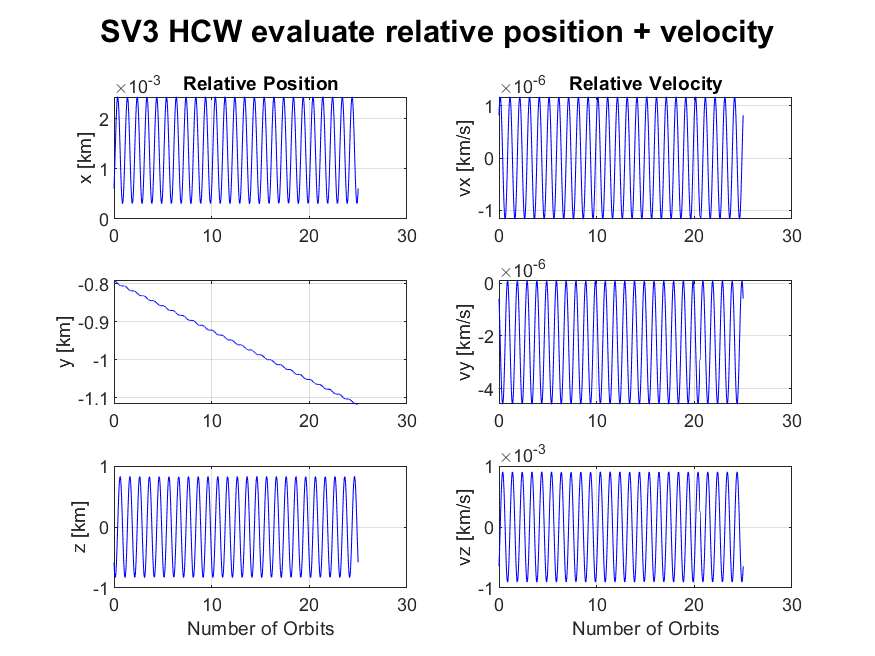
\includegraphics[width=0.7\linewidth]{sim/figures/PS3/HCW_pos_vel_SV2.png}
    \caption{Relative position and velocity of SV2 in the chief's RTN frame, evaluated using HCW equations.}
    \label{fig:hcw_sv2_pos_vel}
\end{figure}

\begin{figure}[htpb]
    \centering
    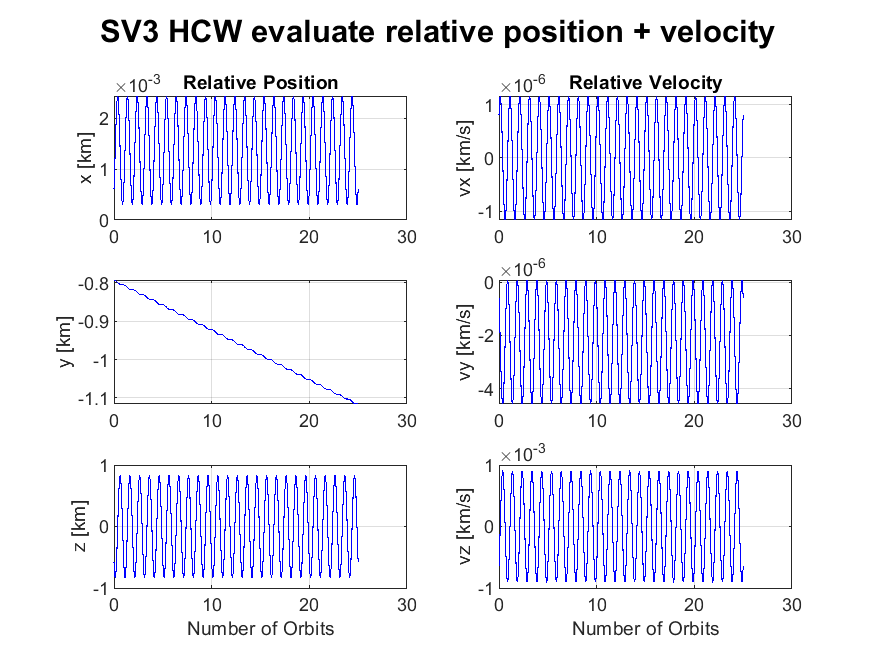
\includegraphics[width=0.7\linewidth]{sim/figures/PS3/HCW_pos_vel_SV3.png}
    \caption{Relative position and velocity of SV3 in the chief's RTN frame, evaluated using HCW equations.}
    \label{fig:hcw_sv2_pos_vel}
\end{figure}

\begin{figure}[htpb]
    \centering
    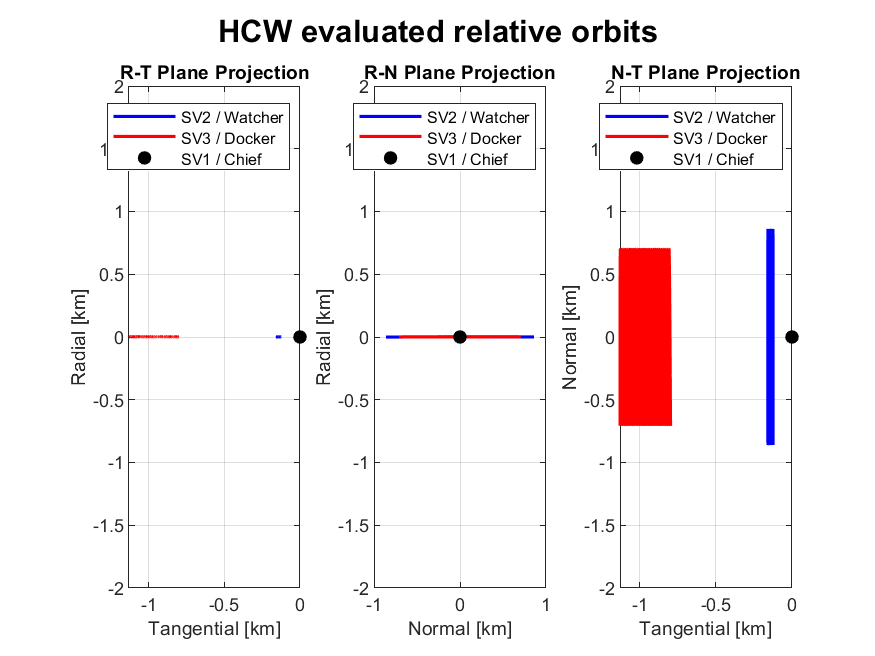
\includegraphics[width=0.7\linewidth]{sim/figures/PS3/RTN_projections_HCW.png}
    \caption{RTN Projections of SV2 and SV3 trajectories calculating using HCW}
    \label{fig:hcw_projections}
\end{figure}

\begin{figure}[htpb]
    \centering
    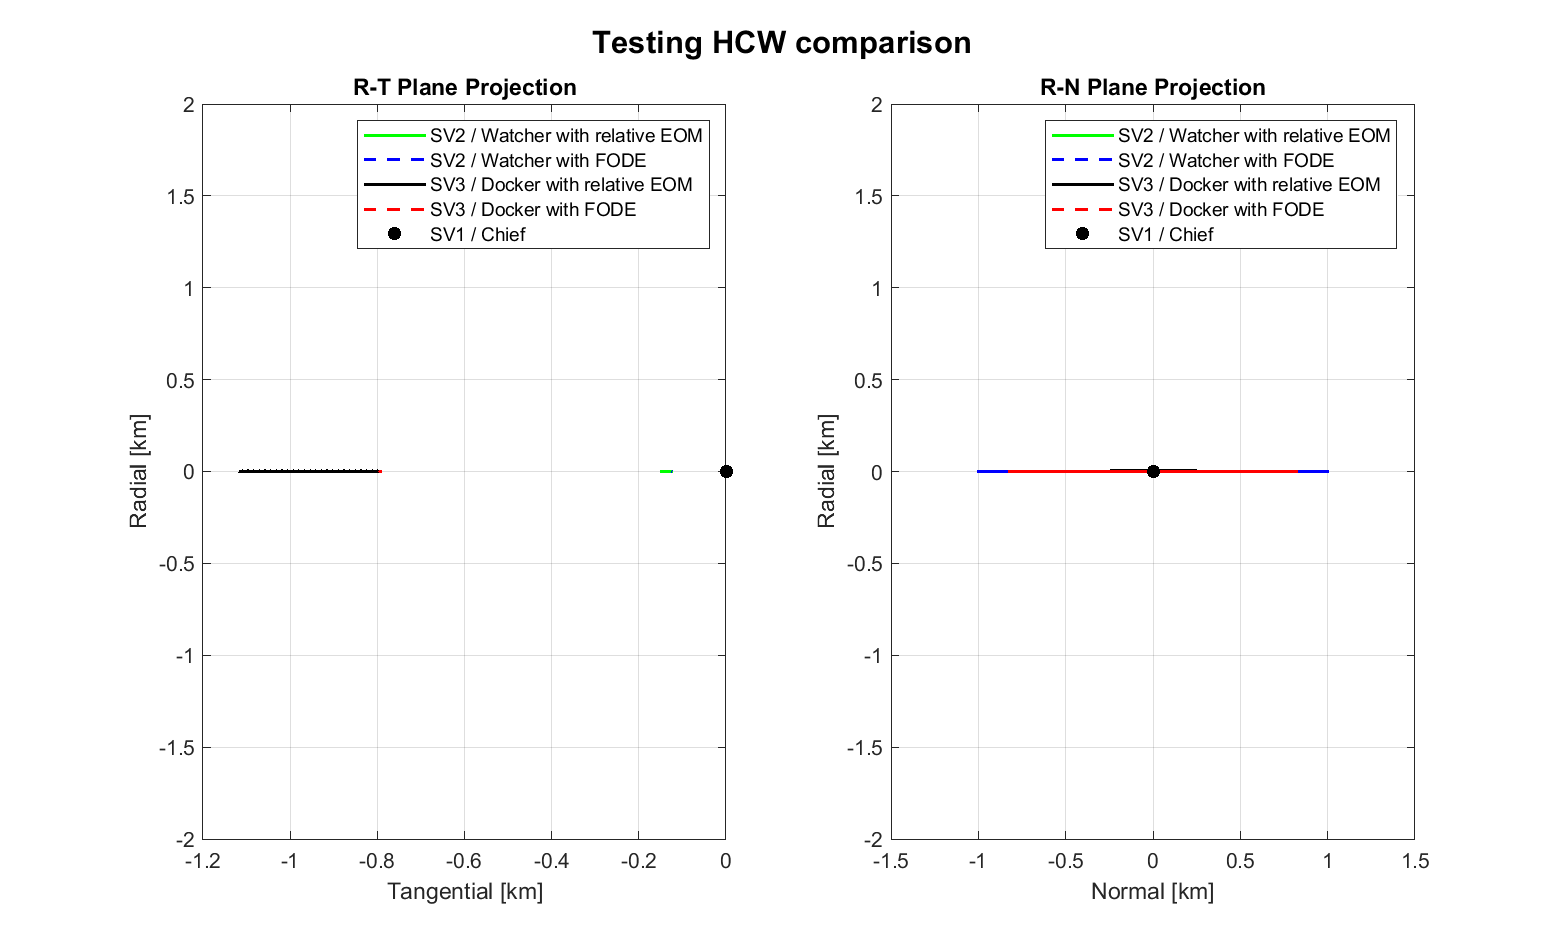
\includegraphics[width=0.7\linewidth]{sim/figures/PS3/RTN_projections_HCW_comparison.png}
    \caption{RTN Projections of SV2 and SV3 comparison between HCW and FERM.}
    \label{fig:hcw_comparisons_projections}
\end{figure}

\begin{figure}[htpb]
    \centering
    \begin{subfigure}[t]{0.45\linewidth}
        \centering
        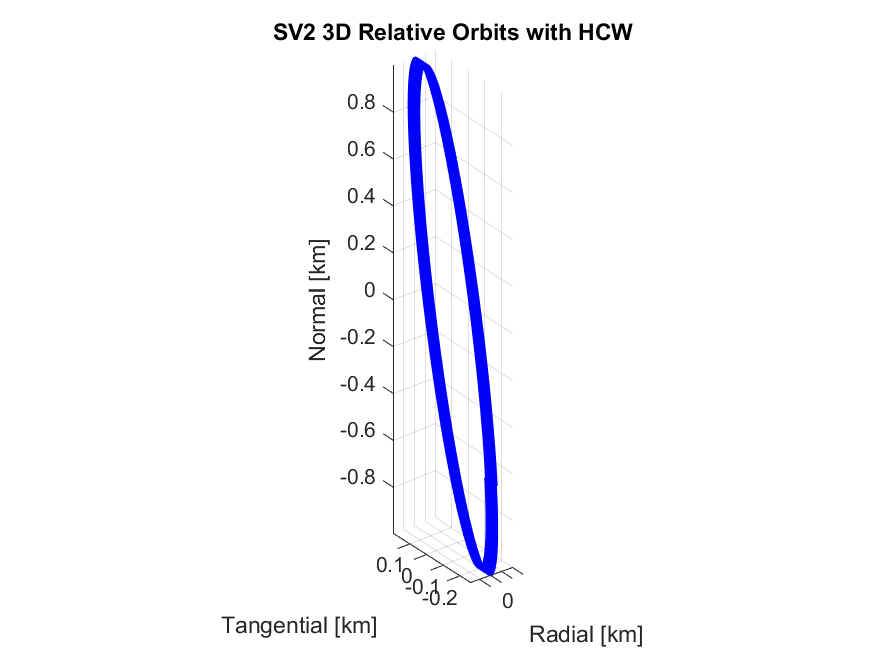
\includegraphics[width=1.2\linewidth]{sim/figures/PS3/3D_HCW_orbit_SV2.png}
        \caption{SV2-HCW Orbit}
        \label{fig:hcw_sv2}
    \end{subfigure}%
    \begin{subfigure}[t]{0.45\linewidth}
        \centering
        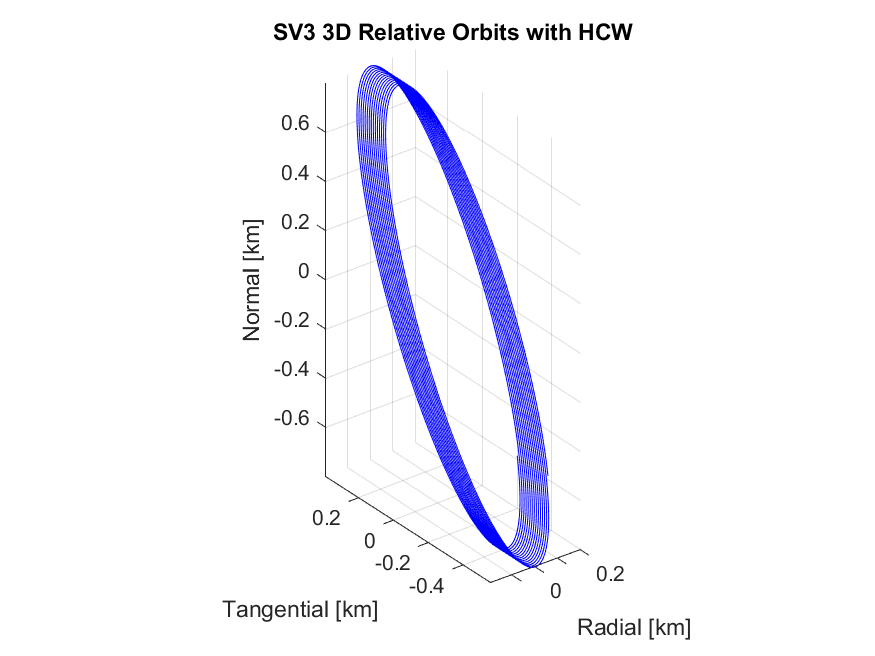
\includegraphics[width=1.2\linewidth]{sim/figures/PS3/3D_HCW_orbit_SV3.png}
        \caption{SV3-HCW Orbit}
        \label{fig:hcw_sv3}
    \end{subfigure}
    \caption{3D HCW-relative orbits of SV2 and SV3.}
    \label{fig:hcw_3d_side_by_side}
\end{figure}

\subsubsection{Analysis of HCW Solution Behavior}

\newpage

\subsection{We are Close in Eccentric Orbits}
\subsubsection{Initial Conditions for Tschauner-Hempel Equations}
Now, we turn our analysis to eccentric orbits, where relative motion is described by the Tschauner-Hempel (TH) equations. The TH equations can be solved using the Yamanaka-Ankersen (YA) model. We will use the same initial conditions for the absolute and relative states as with HCW, except now the chief's orbit has an eccentricity of 0.15. The ROE for SV2 and SV3 remain the same as outlined in Table \ref{{tab:relative_oe_hcw}}, as these initial conditions also lie whtin the range of validity of the TH equations. Specifically, the chief and deputy have equal semi-major axes and the the maximum separation between spacecraft is small relative to the minimum distance from the primary attractor center. 

\subsection{YA Integration Constants}
From these chosen initial conditions, the 6 integration constants of the YA solution can be computed through the following process.

Willis outlines the transformation matrices ($A,B$) from YA integration constants to RTN position and velocity of the deputy \cite{willis2023analytical}. These matrices can be inverted to instead go from initial RTN position and velocity to YA integration constants. 

YA defines the following expressions:
\begin{align*}
n &= \sqrt{\frac{\mu_{\text{earth}}}{a^3}} \\
\eta &= \sqrt{1 - e^2} \\
\tau &= \frac{nt}{\eta^3}\\
k &= 1 + e \cos(f) \\
k' &= -e \sin(f)
\end{align*}

And the following transformation components:
\begin{align*}
\psi_{x1} &= \frac{1}{k} + \frac{3}{2}k' \tau, &
\psi_{x2} &= \sin(f), &
\psi_{x3} &= \cos(f) \\
\psi_{y1} &= -\frac{3}{2}k\tau, &
\psi_{y2} &= \left(1 + \frac{1}{k}\right)\cos(f), &
\psi_{y3} &= -\left(1 + \frac{1}{k}\right)\sin(f), &
\psi_{y4} &= \frac{1}{k} \\
\psi_{z5} &= \frac{1}{k}\sin(f), &
\psi_{z6} &= \frac{1}{k}\cos(f)
\end{align*}

And their respective derivatives:
\begin{align*}
\psi_{x1}' &= \frac{k'}{2} - \frac{3}{2}k^2(k - 1)\tau, &
\psi_{x2}' &= k^2 \cos(f), &
\psi_{x3}' &= -k^2 \sin(f) \\
\psi_{y1}' &= -\frac{3}{2}\left(k + k^2k'\tau\right), &
\psi_{y2}' &= -(k^2 + 1)\sin(f), &
\psi_{y3}' &= -e - (k^2 + 1)\cos(f), &
\psi_{y4}' &= -k' \\
\psi_{z5}' &= e + \cos(f), &
\psi_{z6}' &= -\sin(f)
\end{align*}

And finally the full transformation matrices:
\begin{align*}
A &= 
\begin{bmatrix}
a\eta^2 I_{3 \times 3} & 0 \\
0 & \frac{a n}{\eta} I_{3 \times 3}
\end{bmatrix}
\end{align*}

\begin{align*}
B &=
\begin{bmatrix}
\psi_{x1} & \psi_{x2} & \psi_{x3} & 0 & 0 & 0 \\
\psi_{y1} & \psi_{y2} & \psi_{y3} & \psi_{y4} & 0 & 0 \\
0 & 0 & 0 & 0 & \psi_{z5} & \psi_{z6} \\
\psi_{x1}' & \psi_{x2}' & \psi_{x3}' & 0 & 0 & 0 \\
\psi_{y1}' & \psi_{y2}' & \psi_{y3}' & \psi_{y4}' & 0 & 0 \\
0 & 0 & 0 & 0 & \psi_{z5}' & \psi_{z6}'
\end{bmatrix}
\end{align*}

We then invert the transformation matrices to solve for the initial conditions:
\[
K = (A B)^{-1} \cdot \begin{bmatrix}
x_0 \\ y_0 \\ z_0 \\ \dot{x}_0 \\ \dot{y}_0 \\ \dot{z}_0
\end{bmatrix}
\]

Note that in solving this equation, $\tau$ will be zero because our initial time is 0. For our chosen initial conditions, the integration constants computed are provided in Table \ref{tab:integration_constants_HCW}.

\begin{table}[ht]
    \centering
    \renewcommand{\arraystretch}{1.2}
    \begin{tabular}{c c c}
        \toprule
        \textbf{Constant} & \textbf{SV2} & \textbf{SV3} \\
        \midrule
        $K_1$ & $-1.5886\cdot10^{-8}$ & $-1.0799\cdot10^{-8}$ \\
        $K_2$ & $3.7051\cdot10^{-6}$ & $2.9694\cdot10^{-6}$ \\
        $K_3$ & $-1.4750\cdot10^{-5}$& $-2.9477\cdot10^{-5}$\\
        $K_4$ & $8.4251\cdot10^{-7}$ & $6.7435\cdot10^{-7}$ \\
        $K_5$ & $1.4401\cdot10^{-4}$ & $1.1521\cdot10^{-4}$ \\
        $K_6$ & $3.8971\cdot10^{-8}$ & $3.0781\cdot10^{-8}$ \\
        \bottomrule
    \end{tabular}
    \caption{Integration Constants for SV2 and SV3 Used in HCW Analytical Solution}
    \label{tab:integration_constants_HCW}
\end{table}

\subsection{Relative State Propagation Using YA Solution}
We use the same propagation strategy as with the HCW solution, except now using the YA integration constants and STM. The resulting relative position and velocity in 3D 

